\documentclass[final]{beamer}
\usepackage[orientation=portrait,size=a0,scale=1.3]{beamerposter}
\usetheme{RJH}

\usepackage[utf8]{inputenc}
\usepackage[frenchb]{babel}

\usepackage[absolute,overlay]{textpos}
\setlength{\TPHorizModule}{1cm}
\setlength{\TPVertModule}{1cm}

\title{{\large École Temps-Réel 2015} \\[.3em]
  Implémentation d'un outil de \\
  reconstruction de graphes de flot de contrôle pour \\
  l'analyse temporelle par vérification de modèles}
\author{Armel Mangean \\
  \texttt{armel.mangean@irccyn.ec-nantes.fr}}
\footer{École Centrale de Nantes,
  IRCCyN (équipe Systèmes Temps-Réel)}

\begin{document}
  \begin{frame}

    %%%
    
    \begin{textblock}{39}(2,13)
      \begin{block}{Résumé}\small
        L'analyse temporelle des systèmes embarqués temps-réel est nécessaire
        pour garantir le respect de l'ensemble de leurs contraintes
        temporelles. Une telle analyse doit déterminer si l'ensemble des
        exécutions possibles d'un système respecte l'ensemble des ses
        contraintes temporelles. Les différentes analyses temporelles existantes
        s'appuient conjointement sur le programme et la plateforme matérielle
        considérés.
        \vspace{.5em}
  
        Il est présenté ici l'implémentation d'un outil de génération de modèles
        de programmes adapté à l'analyse temporelle par vérification de
        modèles. Le processus de génération est composé de deux étapes. La
        première réalise une \textit{reconstruction} classique du \textit{graphe
          de flot de contrôle} du programme à partir d'un fichier exécutable. La
        seconde procède à une \textit{réduction} de ce graphe de flot de contrôle
        par \textit{program slicing}.
        \vspace{.4em}
      \end{block}
      \vspace{1em}
      
      \section{Introduction}
      \begin{block}{\thesection. \secname}
        %\begin{itemize}
        %  \item Analyse temporelle
        %  \item Reconstruction de CFG
        %  \item Vérification de modèles
        %\end{itemize}
        
        %\textbf{Worst Case Execution Time}
        \textbf{L'analyse temporelle...}
        \begin{itemize}
          \item[] Le \textit{Worst Case Execution Time (WCET)} d'une tâche est
            la borne supérieure sur les temps d'exécutions de
            celle-ci. Déterminer le WCET d'une tâche est un problème
            difficile. En pratique, il est très souvent utilisé des estimations.
            \vspace{.5em}
          \item[] L'analyse temporelle d'un système temps-réel premet d'obtenir
            des estimations de WCET pour les tâches de ce système. Ces
            estimations de WCET sont issues d'analyses dynamiques (avec
            exécution) ou statiques (sans exécution).
            %La précision de ces
            %estimations est un élément fondamental pour juger de la qualité des
            %différentes analyses.
          %\item[] Le plus couramment, ces analyses ont pour domaine
          %  d'application une tâche isolée du système.
        \end{itemize}
        \vspace{1em}

        \textbf{...par vérification de modèles}
        \begin{itemize}
          \item[] Le \textit{(Timed) Model Checking} consiste en la vérification
            algorithmique de satisfaction d'une propriété (temporelle) par un
            automate (temporisé).

          \item[] L'analyse temporelle par vérification de modèles est une
            analyse statique offrant des possibilités qui n'ont pas encore
            été complétement étudiées.
            \vspace{.5em}
            
            On peut citer :
            \begin{itemize}
              \item[—] l'estimation de WCET avec une précision de l'ordre de la dizaine de cycles ;
              \item[—] l'obtention des valeurs d'entrées associées au WCET estimé ;
              \item[—] l'application de cette analyse à des tâches non-isolées ;
              \item[—] l'estimation équivalente des \textit{Best Case Execution Times}.
            \end{itemize}
          \vspace{.5em}
          \item[] L'analyse temporelle par vérification de modèles souffre
            cependant des limitations inhérente à la vérification de modèles à
            savoir du problème d'explosion de l'espace d'état.
        \end{itemize}
        \vspace{.4em}
      \end{block}
      \vspace{1em}

      %% \section{Travaux connexes}
      %% \begin{block}{\thesection. \secname}
      %%   \begin{itemize}
      %%     \item Approches non-MC
      %%     \item Program Slicing arithmétique
      %%   \end{itemize}
      %%   \vspace{.4em}
      %% \end{block}
      %% \vspace{1em}


      \section{Génération du modèle}
      \begin{block}{\thesection. \secname}
        %\begin{itemize}
        %  \item À partir de fichiers exécutables
        %  \item Analyse sémantique avec HARMLESS
        %  \item Algorithme base de graphes
        %\end{itemize}
        
        \textbf{Le graphe de flot de contrôle}
        \begin{itemize}
          
          \item[] Un bloc de base est une séquence d’instructions qui n’a qu’un
            point d’entrée, sa première instruction, et qu’un point de sortie,
            sa dernière instruction. Le \textit{Control Flow Graph (CFG)} d'un
            tâche est un graphe orienté dans lequel les n{\oe}uds les blocs de
            base du programme et les transitions représentent les enchainements
            possible à l'exécution entre les différents blocs de base du
            programme.
            \vspace{.5em}

          \item[] De manière formelle le CFG d'une tâche est un tuple $(V,E,i)$
            avec $V$ l'ensemble des blocs de base de la tâche, $E \subset V
            \times V$ les chemins du flot de contrôle et $i \in V$ le point
            d'entrée de la tâche.
        \end{itemize}
        \vspace{1em}

        \textbf{Reconstruction de CFG}
        \begin{itemize}
          \item[] La reconstruction de CFG est réalisée en deux étapes. D'abord
            la reconstruction des blocs de base puis la reconstruction des
            chemins du flot de contrôle.
            \vspace{.5em}

            La reconstruction des blocs de base nécessite d'abord d'identifier
            l'ensemble des points d'entrée de blocs de base. Un bloc de base est
            constitué de l'ensemble des instructions entre un point d’entrée
            (inclus) et le point d’entrée suivant (exclus).
            \vspace{.5em}
            
            %Une instruction est une entrée de bloc de base si
            %elle se trouve être :
            %\begin{itemize}
            %  \item[—] le point d’entrée du programme ;
            %  \item[—] une cible de saut ;
            %  \item[—] immédiatement après une instruction de saut ;
            %  \item[—] la première instruction du fichier exécutable.
            %\end{itemize}

            Les chemins de flot de contrôle sont obtenues itérativement en
            associant à chaque bloc de base les cibles possibles de son point de
            sortie. Lorsqu’il n’est pas trivial de déterminer la cible d’un
            saut, comme cela peut l’être dans le cas de sauts indirects. il est
            fait usage de l’outil \textsc{Harmless} [1]. Celui-ci réalise une
            simulation de l’exécution du programme permettant de determiner
            certaines cibles de sauts.
        \end{itemize}
        \vspace{.4em}
      \end{block}
      \vspace{2em}

      %% \begin{itemize}\footnotesize
      %%    \item[] [1] R. Kassem, M. Briday, J.-L. Béchennec, G. Savaton, and
      %%      Y. Trinquet, “Harmless, a hardware architecture description language
      %%      dedicated to real-time embedded system simulation,” Journal of
      %%      Systems Architecture, vol. 58, no. 8, pp. 318–337, Sep. 2012.
      %%    \item[] [2] M. Weiser, “Program Slicing,” in Proceedings of the 5th
      %%      international conference on Software engineering. IEEE Press, 1981,
      %%      pp. 439–449.
      %%    \item[] [3] C. Cifuentes and A. Fraboulet, “Intraprocedural Static
      %%      Slicing of Binary Executables,” in Software Maintenance,
      %%      1997. Proceedings., Internatio- nal Conference on. IEEE, 1997,
      %%      pp. 188–195.
      %%    \item[] [4] K. G. Larsen, P. Pettersson,  and W. Yi, "UPPAAL in a
      %%      Nutshell", International Journal on Software Tools for Technology
      %%      Transfer (STTT) 1.1 (1997): 134-152.
      %%    \item[] [5] S. Marlow. "Haskell 2010 language report", 2010
      %%    \item[] [6] N. Ramsey, J. Dias, and S. Peyton Jones. "Hoopl : a
      %%      modular, reusable library for dataflow analysis and transformation."
      %%      In Proceedings of the 3rd ACM SIGPLAN Symposium on Haskell, Haskell
      %%      2010, Baltimore, MD, USA, 30 September 2010, pages 121–134, 2010.
      %% \end{itemize}

      {\footnotesize
        [1] R. Kassem, M. Briday, J.-L. Béchennec, G. Savaton, and Y. Trinquet,
        “Harmless, a hardware architecture description language dedicated to
        real-time embedded system simulation,” Journal of Systems Architecture,
        vol. 58, no. 8, pp. 318–337, Sep. 2012.  [2] M. Weiser, “Program
        Slicing,” in Proceedings of the 5th international conference on Software
        engineering. IEEE Press, 1981, pp. 439–449.  [3] C. Cifuentes and
        A. Fraboulet, “Intraprocedural Static Slicing of Binary Executables,” in
        Software Maintenance, 1997. Proceedings., Internatio- nal Conference
        on. IEEE, 1997, pp. 188–195.  [4] K. G. Larsen, P. Pettersson, and
        W. Yi, "UPPAAL in a Nutshell", International Journal on Software Tools
        for Technology Transfer (STTT) 1.1 (1997): 134-152.  [5]
        S. Marlow. "Haskell 2010 language report", 2010 [6] N. Ramsey, J. Dias,
        and S. Peyton Jones. "Hoopl : a modular, reusable library for dataflow
        analysis and transformation."  In Proceedings of the 3rd ACM SIGPLAN
        Symposium on Haskell, Haskell 2010, Baltimore, MD, USA, 30 September
        2010, pages 121–134, 2010.
      }
      
    \end{textblock}

    %%%
    
    \begin{textblock}{39}(43,13)
      \section{Réduction du modèle...}
      \begin{block}{\thesection. \secname}
        %\begin{itemize}
        %  \item Program Slicing
        %  \item Réduction de l'éspace d'état
        %\end{itemize}

        \textbf{...par Program Slicing}
        \begin{itemize}
          \item[] Le \textit{Program Slicing} [2,3] permet la réduction d'un programme
            à l'ensemble des instructions affectant l'état de celui-ci à un
            point précis de son exécution. Cette technique peut être utilisée
            pour contenir l'explosion de l'espace d'état dû au modèle logiciel.
            \vspace{.5em}
            
          \item[] En effet, il est suffisant de ne conserver que les états des
            registres influant sur le flot de contrôle dans l'espace d'état afin
            d'y retrouver l'ensemble des exécutions possibles. L'ensemble des
            registres n'influant pas sur le flot de crontôle peut-être déterminé
            par \textit{program slicing} en choissiant pour points d'exécution
            les intructions de contrôle du programme.
            \vspace{.5em}

          \item[] Le fait de ne pas inclure dans l'espace d'état l'ensemble des
            états des registres n'influant pas sur le flot de contrôle du
            programme permet d'en contenir l'explosion.
        \end{itemize}
        %\vspace{1em}

        \begin{figure}
          \centering
          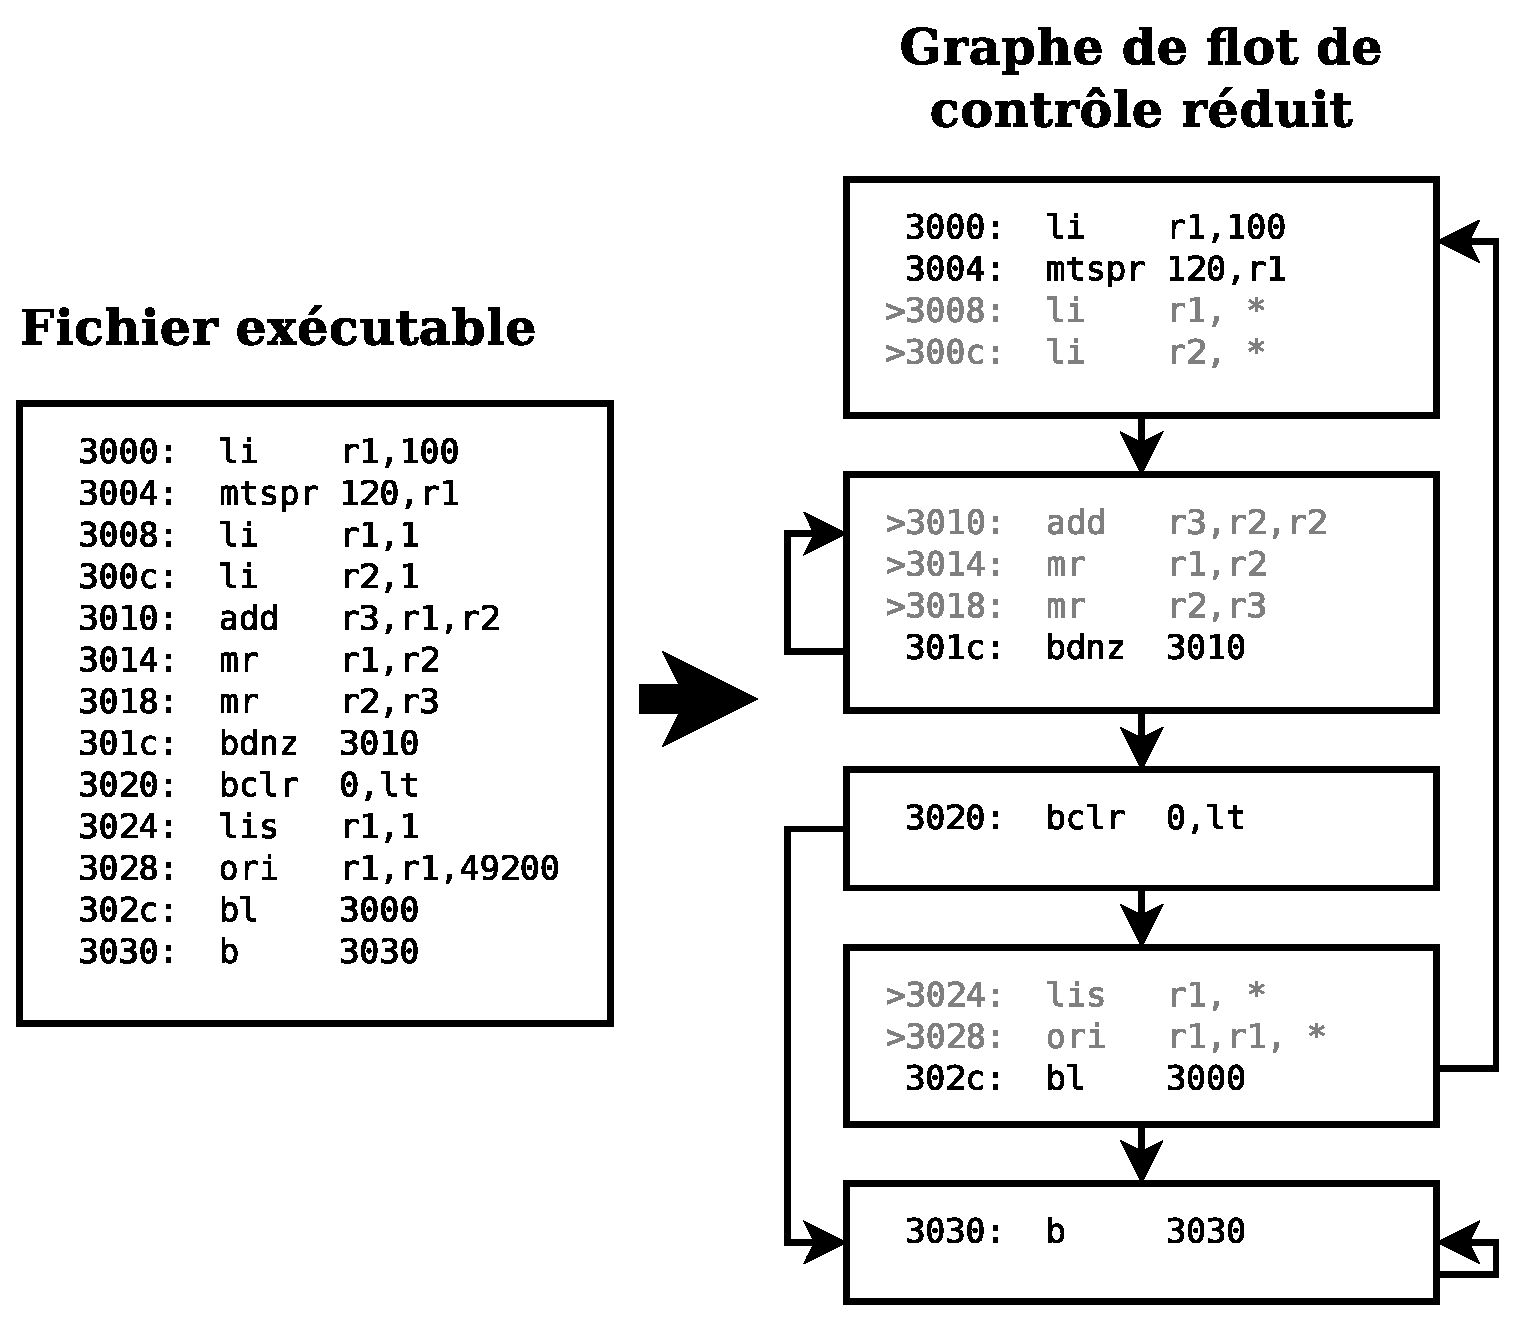
\includegraphics[scale=1]{cfg.eps}
          \caption{Reconstruction et slicing d'un CFG à partir d'un fichier
              exécutable.}
        \end{figure}
        \vspace{.4em}
      \end{block}
      \vspace{1em}

      \section{Implémentation d'un outil}
      \begin{block}{\thesection. \secname}
        \textbf{Fonctionnement de l'outil}
        \begin{itemize}
          \item[] Une analyse sémantique des intructions du fichier exécutable
            est préalablement réalisé grace à l'outil
            \textsc{Harmless}. Celui-ci produit un fichier textuel listant de
            manière ordonnée les instructions du programme.
            \vspace{.5em}

          \item[] L'outil implémenté réalise tout d'abord une analyse syntaxique
            du fichier textuel (\texttt{Parsing} sur la figure). L'algorithme de
            reconstruction de CFG (\texttt{Reconstruction}) puis de réduction de
            celui-ci (\texttt{Slicing}) sont ensuite réalisés.
            \vspace{.5em}
        
        \item[] Le modèle du programme est produit sous forme d'un fichier
          \textsc{XML}. Il peut-être vérifié conjointement avec un modèle d'une
          plateforme matérielle grace à l'outil \textsc{UPPAAL} [4].
        \end{itemize}
        %\vspace{1em}

        \begin{figure}
          \centering
          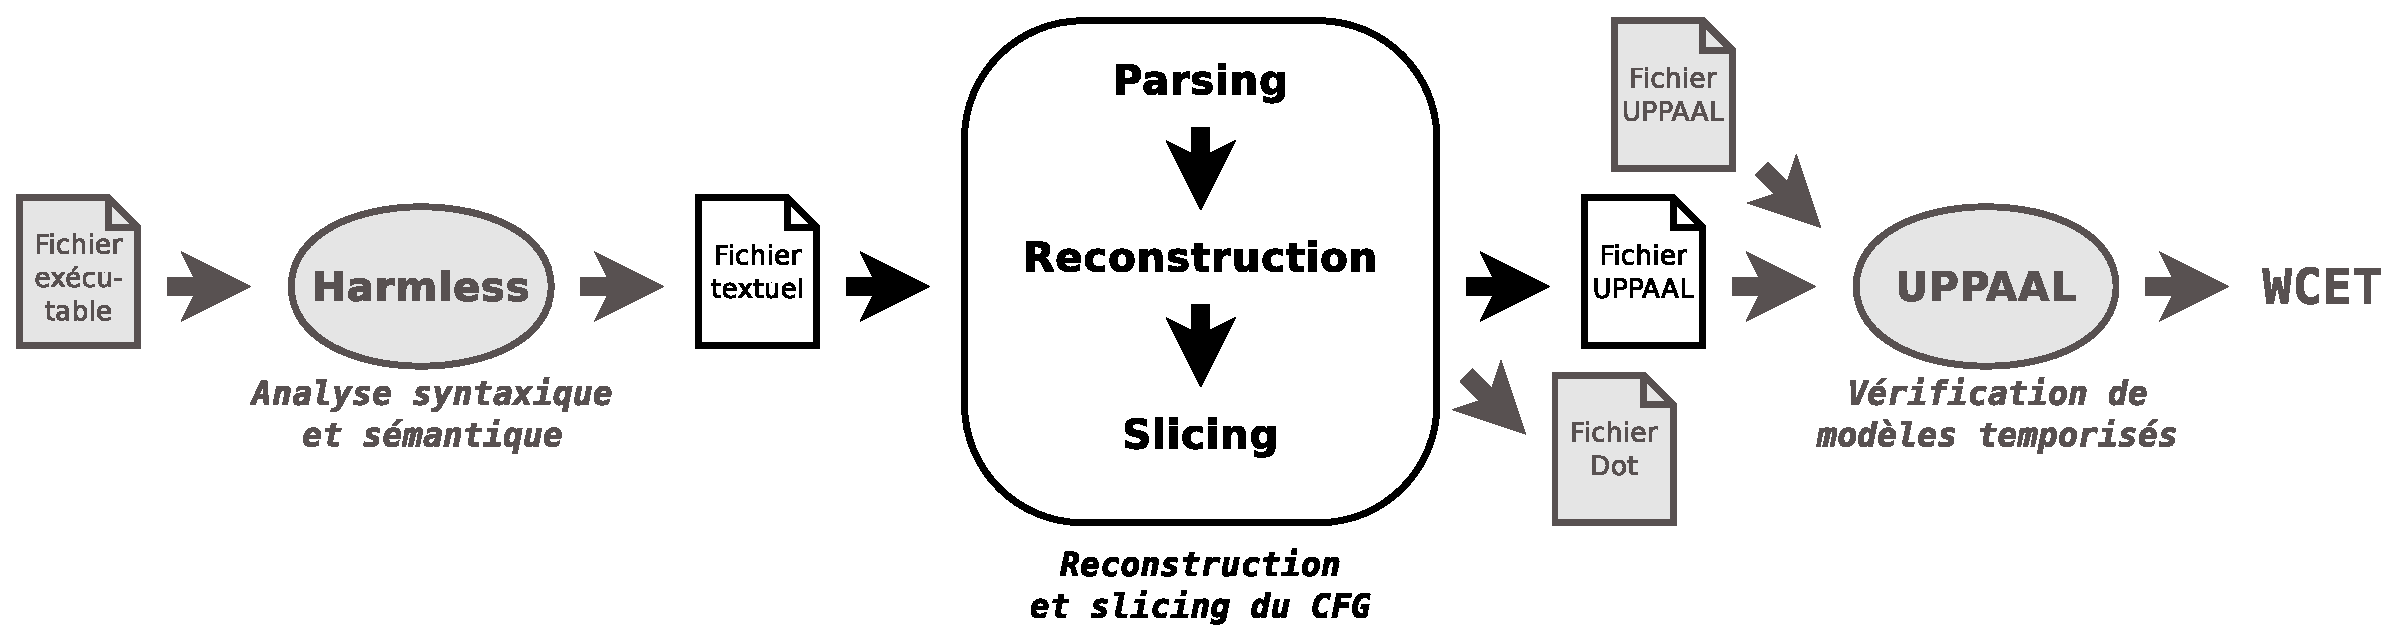
\includegraphics[scale=0.9]{archi.eps}
          \caption{Fonctionnement de l'outil.}
        \end{figure}

        \begin{itemize}
          \item[] L'outil est implémenté en Haskell [5], un langage de programmation
            fonctionnel, grace à Hoopl [6], une bibliothèque de manipulation de
            CFG.
        \end{itemize}

        \vspace{.4em}
      \end{block}
      \vspace{1em}
      
      \section{Conclusion}
      \begin{block}{\thesection. \secname}
        %\begin{itemize}
        %  \item Modélisation matérielle
        %  \item Analyse temporelle
        %\end{itemize}

        \textbf{Travail réalisé}
        \begin{itemize}
          \item[] Implémentation d'un outil de génération automatique de modèles
            logiciels à partir de fichiers exécutable adaptés à l'analyse
            temporelle par vérification de modèles.
        \end{itemize}
        \vspace{1em}
        
        \textbf{Perspectives de travail}
        \begin{itemize}
          \item Poursuite du travail d'implémentation de
            l'outil ;
          \item Production d'un modèle d'une plateforme matérielle
            multi-c{\oe}ur ;
          \item Exploration du potentiel et des limitations de l'analyse
            temporelle par vérification de modèles temporisés.
        \end{itemize}
        \vspace{.4em}
      \end{block}
    \end{textblock}

    %%%
    
  \end{frame}
\end{document}
